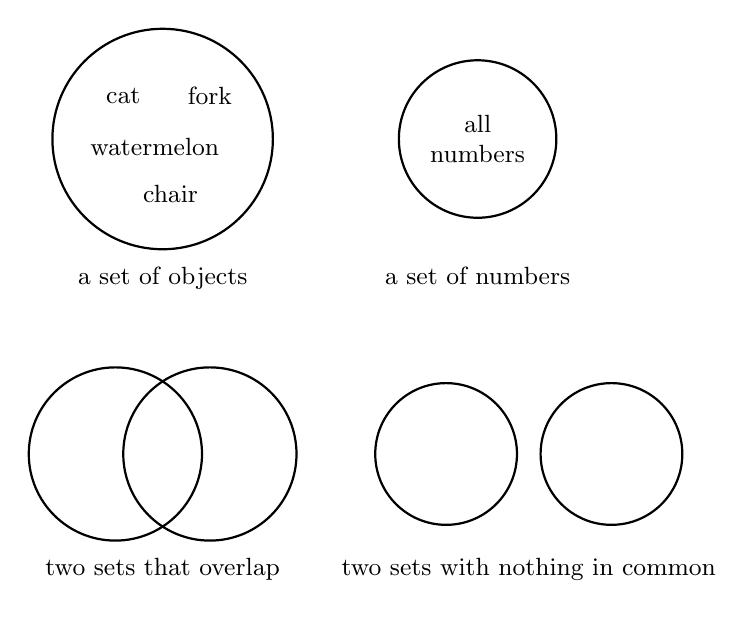
\begin{tikzpicture}[font=\small]
  % a set drawn as a bag of objects
  \draw[thick] (0,0) circle (1.4);
  \node at (-0.5,0.55) {cat};
  \node at (0.6,0.55) {fork};
  \node at (-0.1,-0.1) {watermelon};
  \node at (0.1,-0.7) {chair};
  \node[below] at (0,-1.5) {a set of objects};
  % the set of all numbers
  \draw[thick] (4,0) circle (1.0);
  \node[align=center] at (4,0) {all\\numbers};
  \node[below] at (4,-1.5) {a set of numbers};
  % overlapping sets
  \draw[thick] (-0.6,-4) circle (1.1);
  \draw[thick] (0.6,-4) circle (1.1);
  \node[below] at (0,-5.2) {two sets that overlap};
  % disjoint sets
  \draw[thick] (3.6,-4) circle (0.9);
  \draw[thick] (5.7,-4) circle (0.9);
  \node[below] at (4.65,-5.2) {two sets with nothing in common};
\end{tikzpicture}
